\section{Atividade 7}

\subsection{Análise Avançada do Lugar Geométrico das Raízes (LGR)}

A análise do Lugar Geométrico das Raízes (LGR) fornece insights essenciais sobre a estabilidade e as dinâmicas de resposta do sistema massa-mola-amortecedor, essencial para entender como variações nos parâmetros influenciam o sistema.
\subsection{Código Scilab para simular a resposta do sistema massa-mola-amortecedor}

O código Scilab detalhado abaixo estabelece os parâmetros do sistema, formula a função de transferência correspondente e visualiza o LGR, facilitando a identificação visual de características como estabilidade e comportamento assintótico.

\begin{lstlisting}[language=Scilab, caption=Código Scilab para simular o Lugar geométrico das raízes]
// Definicao dos parametros
M = 10;
C = 7;
K = 5;

// Funcao de transferencia
num = 1;
den = [M, C, K];

// Sistema
sys = syslin('c', num, den);

// Configuracao da cor para o plot do LGR
clf();
sgrid();
evans(sys, 3000, 'red');
\end{lstlisting}

O código acima realiza as seguintes ações:
\begin{itemize}
    \item \textbf{Definição dos parâmetros:} Os valores de \( M \) (massa), \( C \) (coeficiente de amortecimento) e \( K \) (constante da mola) são definidos conforme especificado.
    \item \textbf{Configuração da função de transferência:} A função de transferência do sistema massa-mola-amortecedor é configurada utilizando os parâmetros definidos. O numerador da função de transferência é \(1\), enquanto o denominador é dado por \( [M, C, K] \).
    \item \textbf{Criação do sistema:} O comando \texttt{syslin('c', num, den)} cria a representação do sistema linear contínuo com a função de transferência especificada.
    \item \textbf{Plot do Lugar Geométrico das Raízes:} Os comandos \texttt{clf()}, \texttt{sgrid()}, e \texttt{evans(sys, 3000, 'red')} limpam a figura, desenham uma grade no plano complexo e plota o LGR do sistema, respectivamente. O parâmetro \texttt{3000} especifica o número de pontos de discretização, e \texttt{'red'} define a cor vermelha para as curvas do LGR.
\end{itemize}

Este código é fundamental para visualizar como os pólos do sistema variam com mudanças nos parâmetros, permitindo uma análise detalhada da estabilidade e do comportamento dinâmico do sistema massa-mola-amortecedor.

\begin{figure}[h]
    \centering
    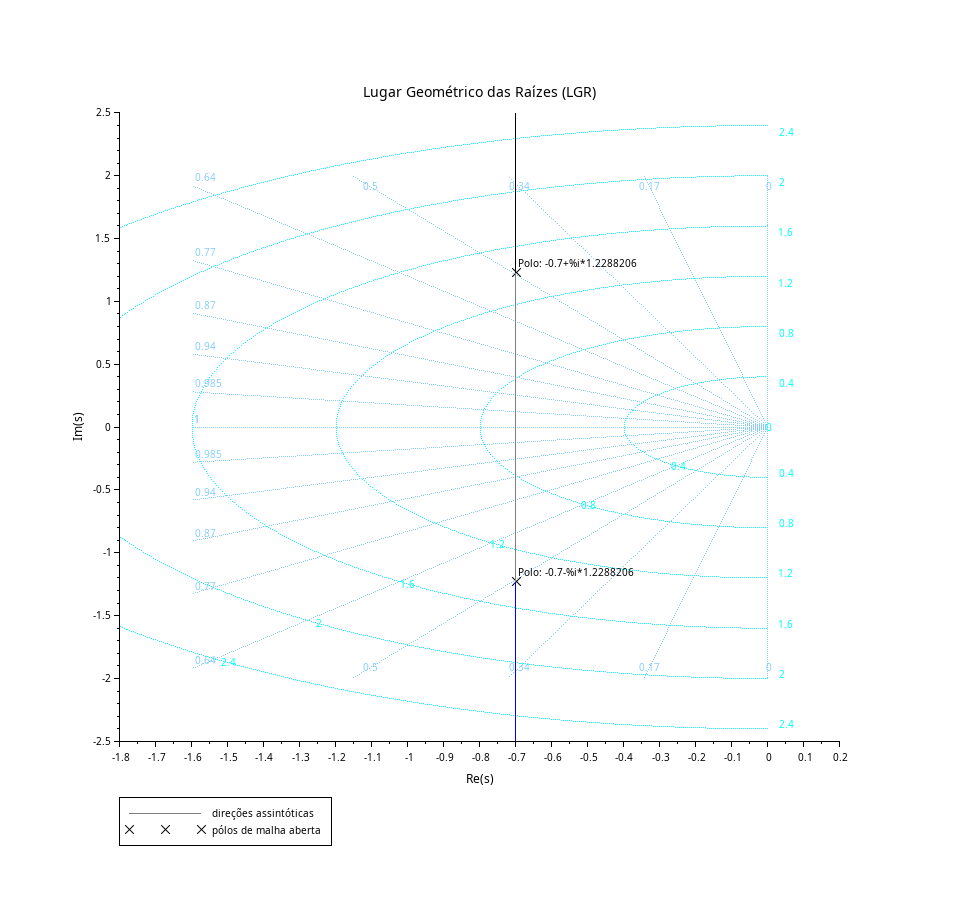
\includegraphics[width=0.8\textwidth]{atividades/7-atividade/assets/lgr.png}
    \caption{Lugar Geométrico das Raízes do sistema massa-mola-amortecedor.}
    \label{fig:LGR}
\end{figure}

Esta análise do Lugar Geométrico das Raízes (LGR) sugere uma tendência do sistema de manter a estabilidade diante de variações nos parâmetros, embora essa interpretação dependa de suposições sobre as condições de contorno e a natureza das mudanças paramétricas. As propriedades observadas nos pólos e nas assíntotas, particularmente sua simetria, fornecem indícios importantes para o design de sistemas de controle. No entanto, é essencial considerar que a visualização por meio do LGR oferece uma perspectiva limitada, que precisa ser complementada com outras análises dinâmicas para validar completamente a estabilidade e a eficácia do controle em cenários variados.

\begin{itemize}
    \item \textbf{Pólos e Simetria:}
          Os pólos do sistema são localizados em \( s = -0.7 \) e \( s = -1.2 \) indicam uma resposta sem oscilações significativas devido ao posicionamento no semiplano esquerdo, caracterizando uma estabilidade inerente. Essa configuração em torno do eixo real indica que os pólos são reais e negativos, o que implica que o sistema não exibe comportamento oscilatório significativo. A simetria sugere que a resposta do sistema será caracterizada por um amortecimento subcrítico, estabilizando-se sem oscilações.

    \item \textbf{Estabilidade e Assíntotas:}
          O sistema não possui zeros e tem dois pólos, indicando que o número de assíntotas é igual ao número de pólos menos o número de zeros, resultando em duas assíntotas. Estas assíntotas são calculadas pela fórmula \[
              \alpha_k = \frac{(2k + 1) \cdot 180^\circ}{2},
          \] resultando em \( \alpha_0 = 90^\circ \) e \( \alpha_1 = -90^\circ \) ou \( 270^\circ \). As assíntotas calculadas, verticais neste caso, preveem que aumentos no ganho do controlador resultarão em movimento vertical dos pólos no plano complexo, preservando a estabilidade enquanto não cruzarem o eixo imaginário.

    \item \textbf{Considerações sobre a Estabilidade:}
          A localização completa dos pólos no semiplano esquerdo confirma a estabilidade do sistema em malha aberta. A análise sugere que o sistema mantém sua estabilidade para os intervalos de ganhos examinados. No entanto, recomenda-se uma investigação adicional, utilizando técnicas como a análise de Nyquist ou Bode, para confirmar essas observações sob uma gama mais ampla de variações paramétricas.
\end{itemize}


